\documentclass{article}
\usepackage[utf8]{inputenc}
\usepackage[english]{babel}
\usepackage[]{amsthm}
\usepackage[]{amssymb}
\usepackage[]{amsmath}
\usepackage[]{hyperref}
\usepackage[]{cancel}
\usepackage[]{graphicx}
\usepackage[]{xcolor}
\usepackage[]{tabularx}
\usepackage[]{fancyhdr}
\hypersetup{
    colorlinks,
    linkcolor={red!50!black},
    citecolor={blue!50!black},
    urlcolor={blue!80!black}
}

\pagestyle{fancy}
\fancyhf{}
\title{\vspace{-4cm}MTH30002 - Differential Equations Assignment 10}
\author{Joshua Rogers}
\lhead{MTH30002 Assignment 10}
\rhead{Joshua Rogers 101096819}
\date\today

\begin{document}
\maketitle
\section*{Exercise 4.8}

\begin{align*}
& u(x,y) = X(x)Y(y) \\
& 0 = \frac{d^2u}{dx^2} + \frac{d^2u}{dy^2}
\end{align*}

Combining these two equations gives us

$$-\frac{1}{X} \frac{d^2X}{dX^2} = (-k^2 = \lambda) = \frac{1}{Y} \frac{d^2Y}{dY^2}$$
where $\lambda = -k^2$ for ease-of-use.

\begin{align*}
\frac{d^2X}{dx^2} + \lambda X =0: &C\sin(\sqrt\lambda x) + D\cos(\sqrt\lambda x)\\
\frac{d^2Y}{dy^2}-\lambda y=0: &Ae^{\sqrt\lambda y} + Be^{-\sqrt\lambda y}
\end{align*}

With the following conditions
$X(0) = X(24) = 0$ we have

\begin{align*}
&C\sin(0) + D\cos(0) = 0\\
&\sin(\sqrt\lambda 24) + D\cos(\sqrt\lambda 24) =0
\end{align*}

$$\det \left( \begin{bmatrix} 0 & 1 \\ \sin(\sqrt\lambda 24) & ... \end{bmatrix} \right) = 0 \Bigr| \lambda \neq 0 $$

\begin{align*}
&-\sin(\sqrt\lambda 24)=0\\
& \therefore \lambda_n = \left(\frac{\pi \cdot n}{24}\right)^2
\end{align*}

$X(0) = C\sin(0)$ thus we have

$$X_n(x) = C_n\sin\left(\frac{\pi \cdot n \cdot x}{24}\right)\Bigr| n\geq 1$$

Given the conditions $Y(24)=20$ and $Y(0)=0$, and the $\lambda_n$ we have, we conclude
$$Y_n=B_n\sinh\left(\sqrt\lambda y\right)$$

Thus, we have

$$u_n(x,y) = E_n\sinh\left(\frac{\pi n y}{24}\right) \sin\left(\frac{\pi n x}{24}\right)\Bigr| n \geq 1, E_n = C_n \cdot B_n$$

$$u(x,y) = \sum_{n=1}^{\infty} \left( E_n \sinh\left(\frac{\pi n y}{24}\right)\right)\sin\left(\frac{\pi n x}{24}\right)$$


This is clearly the odd expansion fourier series of a function, $f(x)$ with
$$b_n = E_n \cdot \sinh\left(\frac{\pi n y}{24}\right) = \frac{2}{24} \int_0^{24} f(x) \sin\left(\frac{n \pi x}{24}\right) dx$$

$$E_n = \frac{2}{24} \cdot \sinh^{-1}\left(\frac{\pi n y}{24}\right) \int_0^{24} f(x) \sin\left(\frac{n \pi x}{24}\right) dx$$



Given $u(x,24) = 20$, we have

$$20 = \sum_{n=1}^{\infty} \left( E_n \sinh(n \pi)\right)\sin\left(\frac{\pi n x}{24}\right)$$

$$E_n = \frac{2}{24} \cdot \sinh^{-1}\left(\pi n\right) \int_0^{24} 20 \sin\left(\frac{n \pi x}{24}\right) dx =  \frac{40(1-\cos(\pi n))}{\pi n\sinh(\pi n)}$$
or rather
$$E_n = \frac{40(1-(-1)^n)}{\pi n \cdot \sinh(\pi n)}$$
which is zero for all even values of $n$.

Thus, we have

$$E_{2n} = 0$$
$$E_{2n-1} = \frac{80}{\pi (2n-1) \cdot \sinh(\pi (2n-1))}$$


Thus we have the beautiful equation

$$u\left(x,y\right)=\sum_{n=1}^{\infty}\frac{80}{\pi\left(2n-1\right)\\sinh\left(\left(2n-1\right)\pi\right)}\\sinh\left(\frac{\left(2n-1\right)\pi y}{24}\right)\\sin\left(\frac{\left(2n-1\right)\pi x}{24}\right)$$

For fun, we graph this using octave using the $\href{https://skill-lync.com/projects/Solving-the-steady-and-unsteady-2D-heat-conduction-problem-using-Matlab-99440}{Jacobi}$ method algorithm.

\begin{figure}
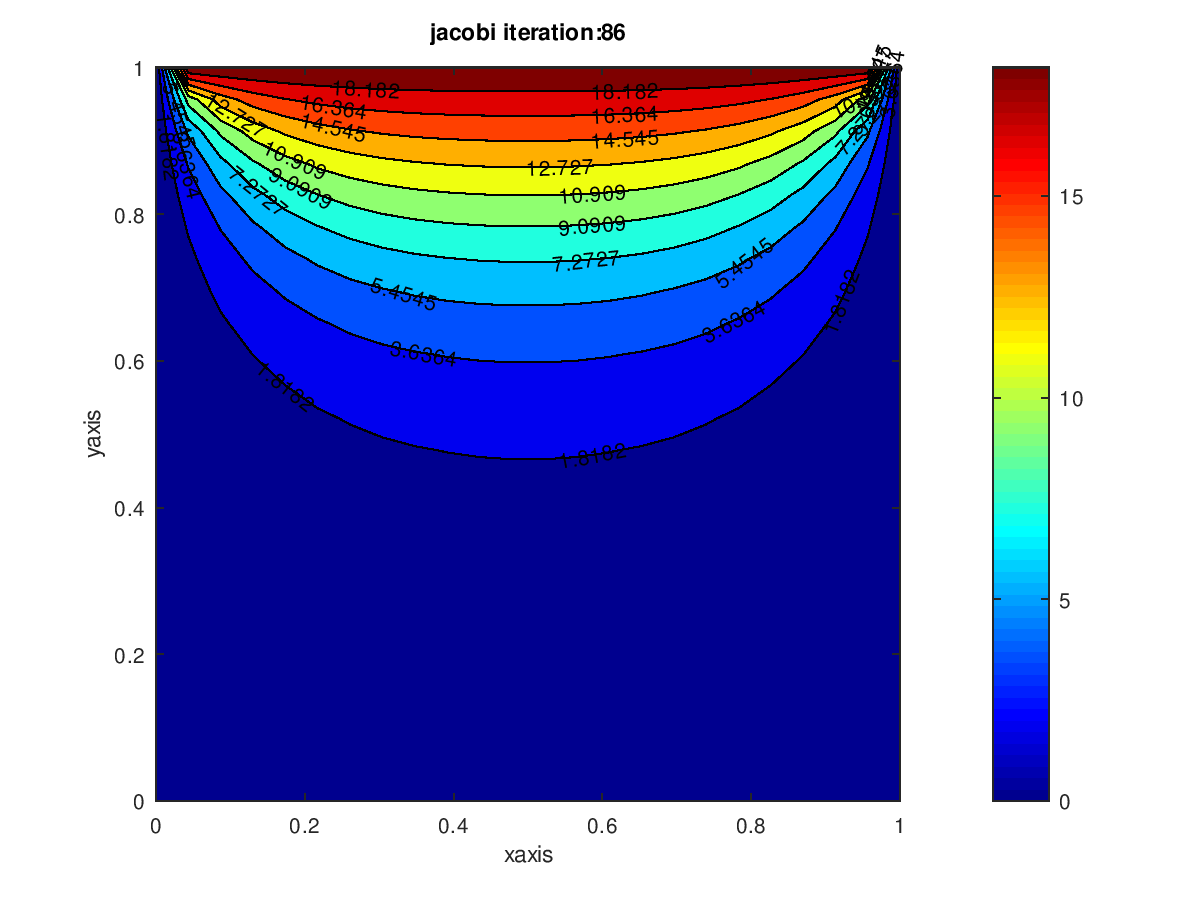
\includegraphics[width=1.0\textwidth]{./static/Jacobi.png}
\caption{Steady state u(x,y)}
\end{figure}

\section*{Exercise 5.1}

\begin{align*}
B_{mn} &= \frac{4}{ab} \int_0^b \int_0^a k \sin \left( \frac{m\pi x}{a}\right) \sin\left( \frac{n \pi y}{b}\right) dx dy\\
= \frac{4k}{ab} \int_0^b \int_0^a ... \\
= \frac{16k}{\pi^2 m n} \cdot \sin^2\left(\frac{\pi m}{2}\right) \cdot \sin^2\left(\frac{\pi n}{2}\right)
\end{align*}

For even numbers of $n$ or $m$ this is zero.

$$B_{2m,2n} = 0$$
$$B_{2m-1,2n-1} = \frac{16k}{\pi^2(2m-1)(2n-1)}$$

Thus, we have the solution

$$u(x,y,0) = f(x,y) = k = \sum_{m=1}^{\infty} \sum_{n=1}^{\infty} \frac{16k}{\pi^2(2m-1)(2n-1)} \sin\left(\frac{(2m-1)\pi x}{a}\right)\sin\left(\frac{(2n-1)\pi y}{b}\right)$$


\section*{Exercise 5.2}

$$u(t,x,y) = T(t)X(x)Y(y)$$
\begin{align*}
\frac{1}{c^2}\frac{T''}{T}=\frac{X''}{X}+\frac{Y''}{Y} \\
\frac{1}{c^2}\frac{T''}{T}=A= \frac{X''}{X}+\frac{Y''}{Y}
\end{align*}

Thus
\begin{align*}
T^{''}-c^2AT=0
\end{align*}

And

\begin{align*}
\frac{X^{''}}{X} = - \frac{Y^{''}}{Y} + A\\
\frac{X^{''}}{X} = B = - \frac{Y^{''}}{Y} + A
\end{align*}

Let $C = A-B$:
\begin{align*}
&X^{''} - BX=0\\
&Y^{''} - CY=0
\end{align*}

From previous studies, we know the eigenvalues and eigenfuctions for $X(x)$ and $Y(y)$ are

\begin{align*}
&X_m(x) = \sin\left( \mu_mx\right), & \mu_m = \frac{m\pi}{a}\Bigr| m \geq 1\\
&Y_n(y) = \sin\left( \nu_ny\right), & \nu_n = \frac{n\pi}{b}\Bigr| n \geq 1
\end{align*}

Given this, and for the specified separatin constants and eigenfunctions to 'hold', we have

$$A=B+C=-(\mu_m^2+\nu_n^2) <0$$

Thus,

$$T_{mn}(t)=D_{mn}\cos\left(\lambda_{mn}t\right)+E_{mn}\sin\left(\lambda_{mn}t\right)$$

Given the initial velocity is 0, we thus have

$$T_{mn}(t)=D_{mn}\cos\left(\lambda_{mn}t\right)$$

$$\lambda_{mn}=c \pi \sqrt{\frac{m^2}{a^2}+\frac{n^2}{b^2}}\Bigr| m,n \geq 1$$

$$u(t,x,y) = \sum_{n=1}^{\infty} \sum_{m=1}^{\infty} D_{mn}\cos\left(c\sqrt{\mu_m^2 + \nu_n^2}t\right) \sin\left( \mu_mx\right) \sin\left( \nu_ny\right)\Bigr|\mu_m = \frac{m\pi}{a}, \nu_n = \frac{n \pi}{b}, [m,n]\geq 1$$


Given the initial deflection, we have
$$u(x,y,t) = \sin\left(\frac{3\pi x}{a}\right)\sin\left(\frac{4\pi y}{b}\right) = \sum_{m=1}^{\infty} \sum_{n=1}^{\infty} D_{m,n}\sin\left( \frac{m\pi}{a} x\right) \sin\left( \frac{n \pi}{b} y\right)$$

This implies that $D_{3,4}$ is the only non-zero solution is equal to $1$.

$$u(x,y,t) = \cos\left(t \cdot \sqrt{ \left(\frac{3 \pi}{a}\right)^2 + \left(\frac{4 \pi}{b}\right)^2}\right)\sin\left(\frac{3x\pi}{a}\right)\sin\left(\frac{4y\pi}{b}\right)$$
or rather,
$$u(x,y,t) = \cos\left(t \pi \cdot \sqrt{ \left(\frac{9}{a^2}\right) + \left(\frac{16 \pi}{b^2}\right)}\right)\sin\left(\frac{3x\pi}{a}\right)\sin\left(\frac{4y\pi}{b}\right)$$

\end{document}
